\documentclass[10pt,a4paper]{article}

\usepackage[utf8]{inputenc}
\usepackage[T1]{fontenc}
\usepackage{babel}
\usepackage[margin=1.6cm, top=1.4cm, bottom=1.4cm, headheight=14pt]{geometry}
\usepackage{xcolor}
\usepackage{enumitem}
\usepackage{titlesec}
\usepackage{fancyhdr}
\usepackage{graphicx}
\usepackage{tabularx}
\usepackage{booktabs}
\usepackage{microtype}
\usepackage{helvet}
\renewcommand{\familydefault}{\sfdefault}

\definecolor{accent}{RGB}{30, 80, 162}
\definecolor{muted}{RGB}{120, 120, 120}
\definecolor{rule}{RGB}{210, 215, 225}

\setlength{\parskip}{2pt}
\setlength{\parindent}{0pt}

% Header
\pagestyle{fancy}
\fancyhf{}
\fancyhead[L]{\small\color{muted} Système de Gestion de Flotte \enspace\textbar\enspace ADR Semaine 1}
\fancyhead[R]{\small\color{muted} 11 mars 2026}
\fancyfoot[C]{\small\color{muted}\thepage}
\renewcommand{\headrulewidth}{0pt}

% Sections : numéro en bleu + texte normal
\titleformat{\section}
  {\normalsize\bfseries\color{accent}}{}{0em}{}[\ \textcolor{rule}{\rule[0.5ex]{0.3\linewidth}{0.4pt}}]
\titlespacing{\section}{0pt}{10pt}{6pt}

\newcommand{\ruledline}{\textcolor{rule}{\rule{\linewidth}{0.4pt}}\vspace{4pt}}

\begin{document}


\begin{titlepage}
  \centering
  \vspace*{3cm}
  {\LARGE\bfseries UNIVERSITÉ DE ROUEN NORMANDIE\\[4pt]
  FACULTÉ DES SCIENCES ET TECHNIQUES\par}
  \vspace{2cm}
  {\large ANNÉE UNIVERSITAIRE 2025--2026\par}
  \vspace{2cm}
  \textcolor{rule}{\rule{\textwidth}{1.5pt}}
  \vspace{1cm}

  {\huge\bfseries\color{accent} Architecture Decision Records\par}
  \vspace{0.4cm}
  {\Large Système de Gestion de Flotte\par}
  \vspace{0.4cm}
  {\large Semaine 1\par}

  \vspace{1cm}
  \textcolor{rule}{\rule{\textwidth}{1.5pt}}
  \vfill
  {\small 11 mars 2026}
\end{titlepage}

\tableofcontents
\newpage

% ---- EN-TÊTE ----
{\fontsize{16}{20}\selectfont\bfseries\color{accent} Architecture Decision Records}\\[2pt]
{\large Système de Gestion de Flotte}\\[4pt]
\ruledline

{\small Le projet consiste à construire un système de \textbf{suivi en temps réel d'une flotte de véhicules}, incluant la gestion des conducteurs, des maintenances et des alertes automatiques. Les utilisateurs sont les administrateurs, managers et techniciens/conducteurs.}
\vspace{3pt}

% ---- DIAGRAMMES ----
\begin{minipage}[t]{0.30\linewidth}
  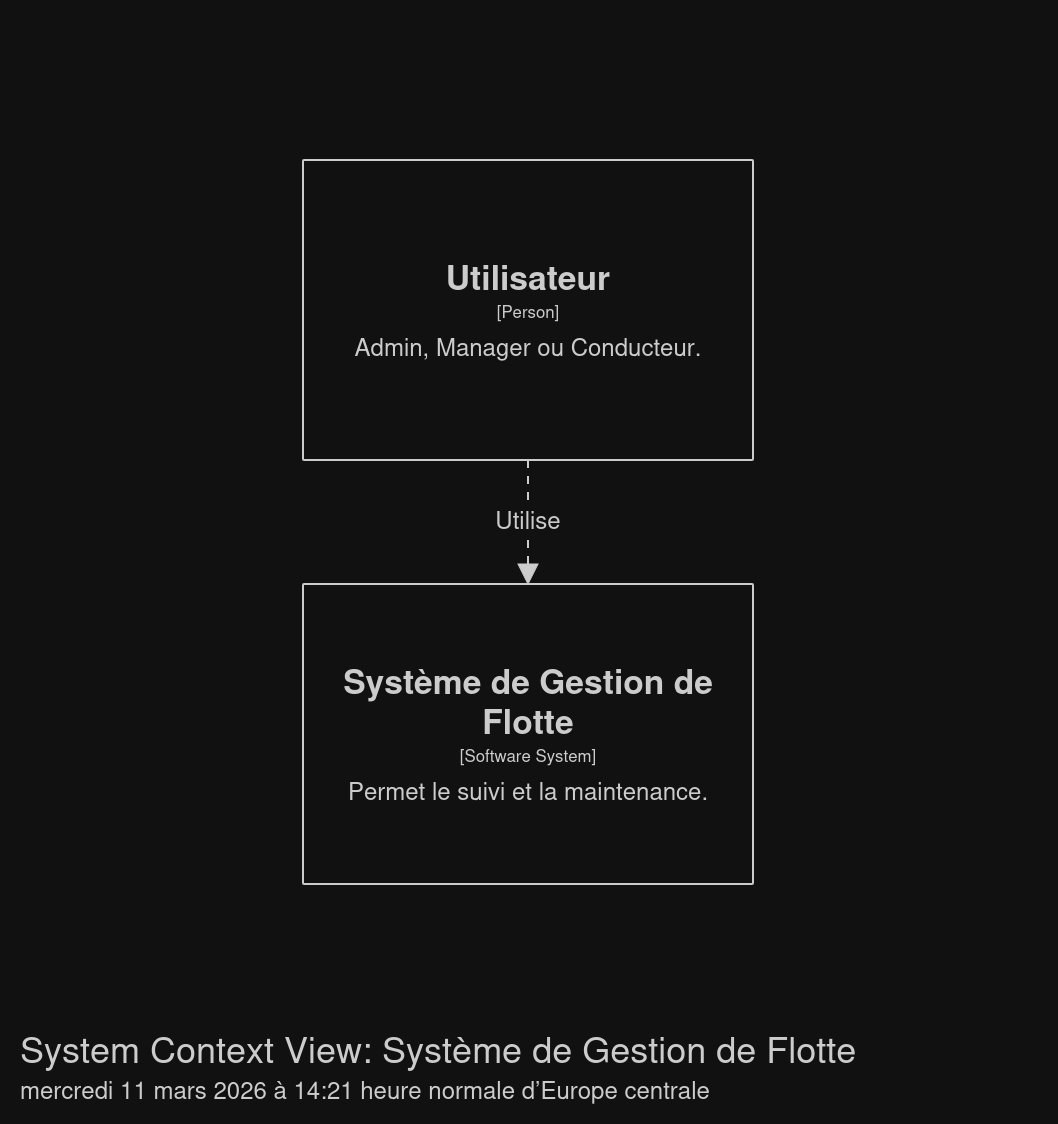
\includegraphics[width=0.95\linewidth]{C1.png}
  \centering{\tiny\color{muted} Vue système}
\end{minipage}
\hfill
\begin{minipage}[t]{0.65\linewidth}
  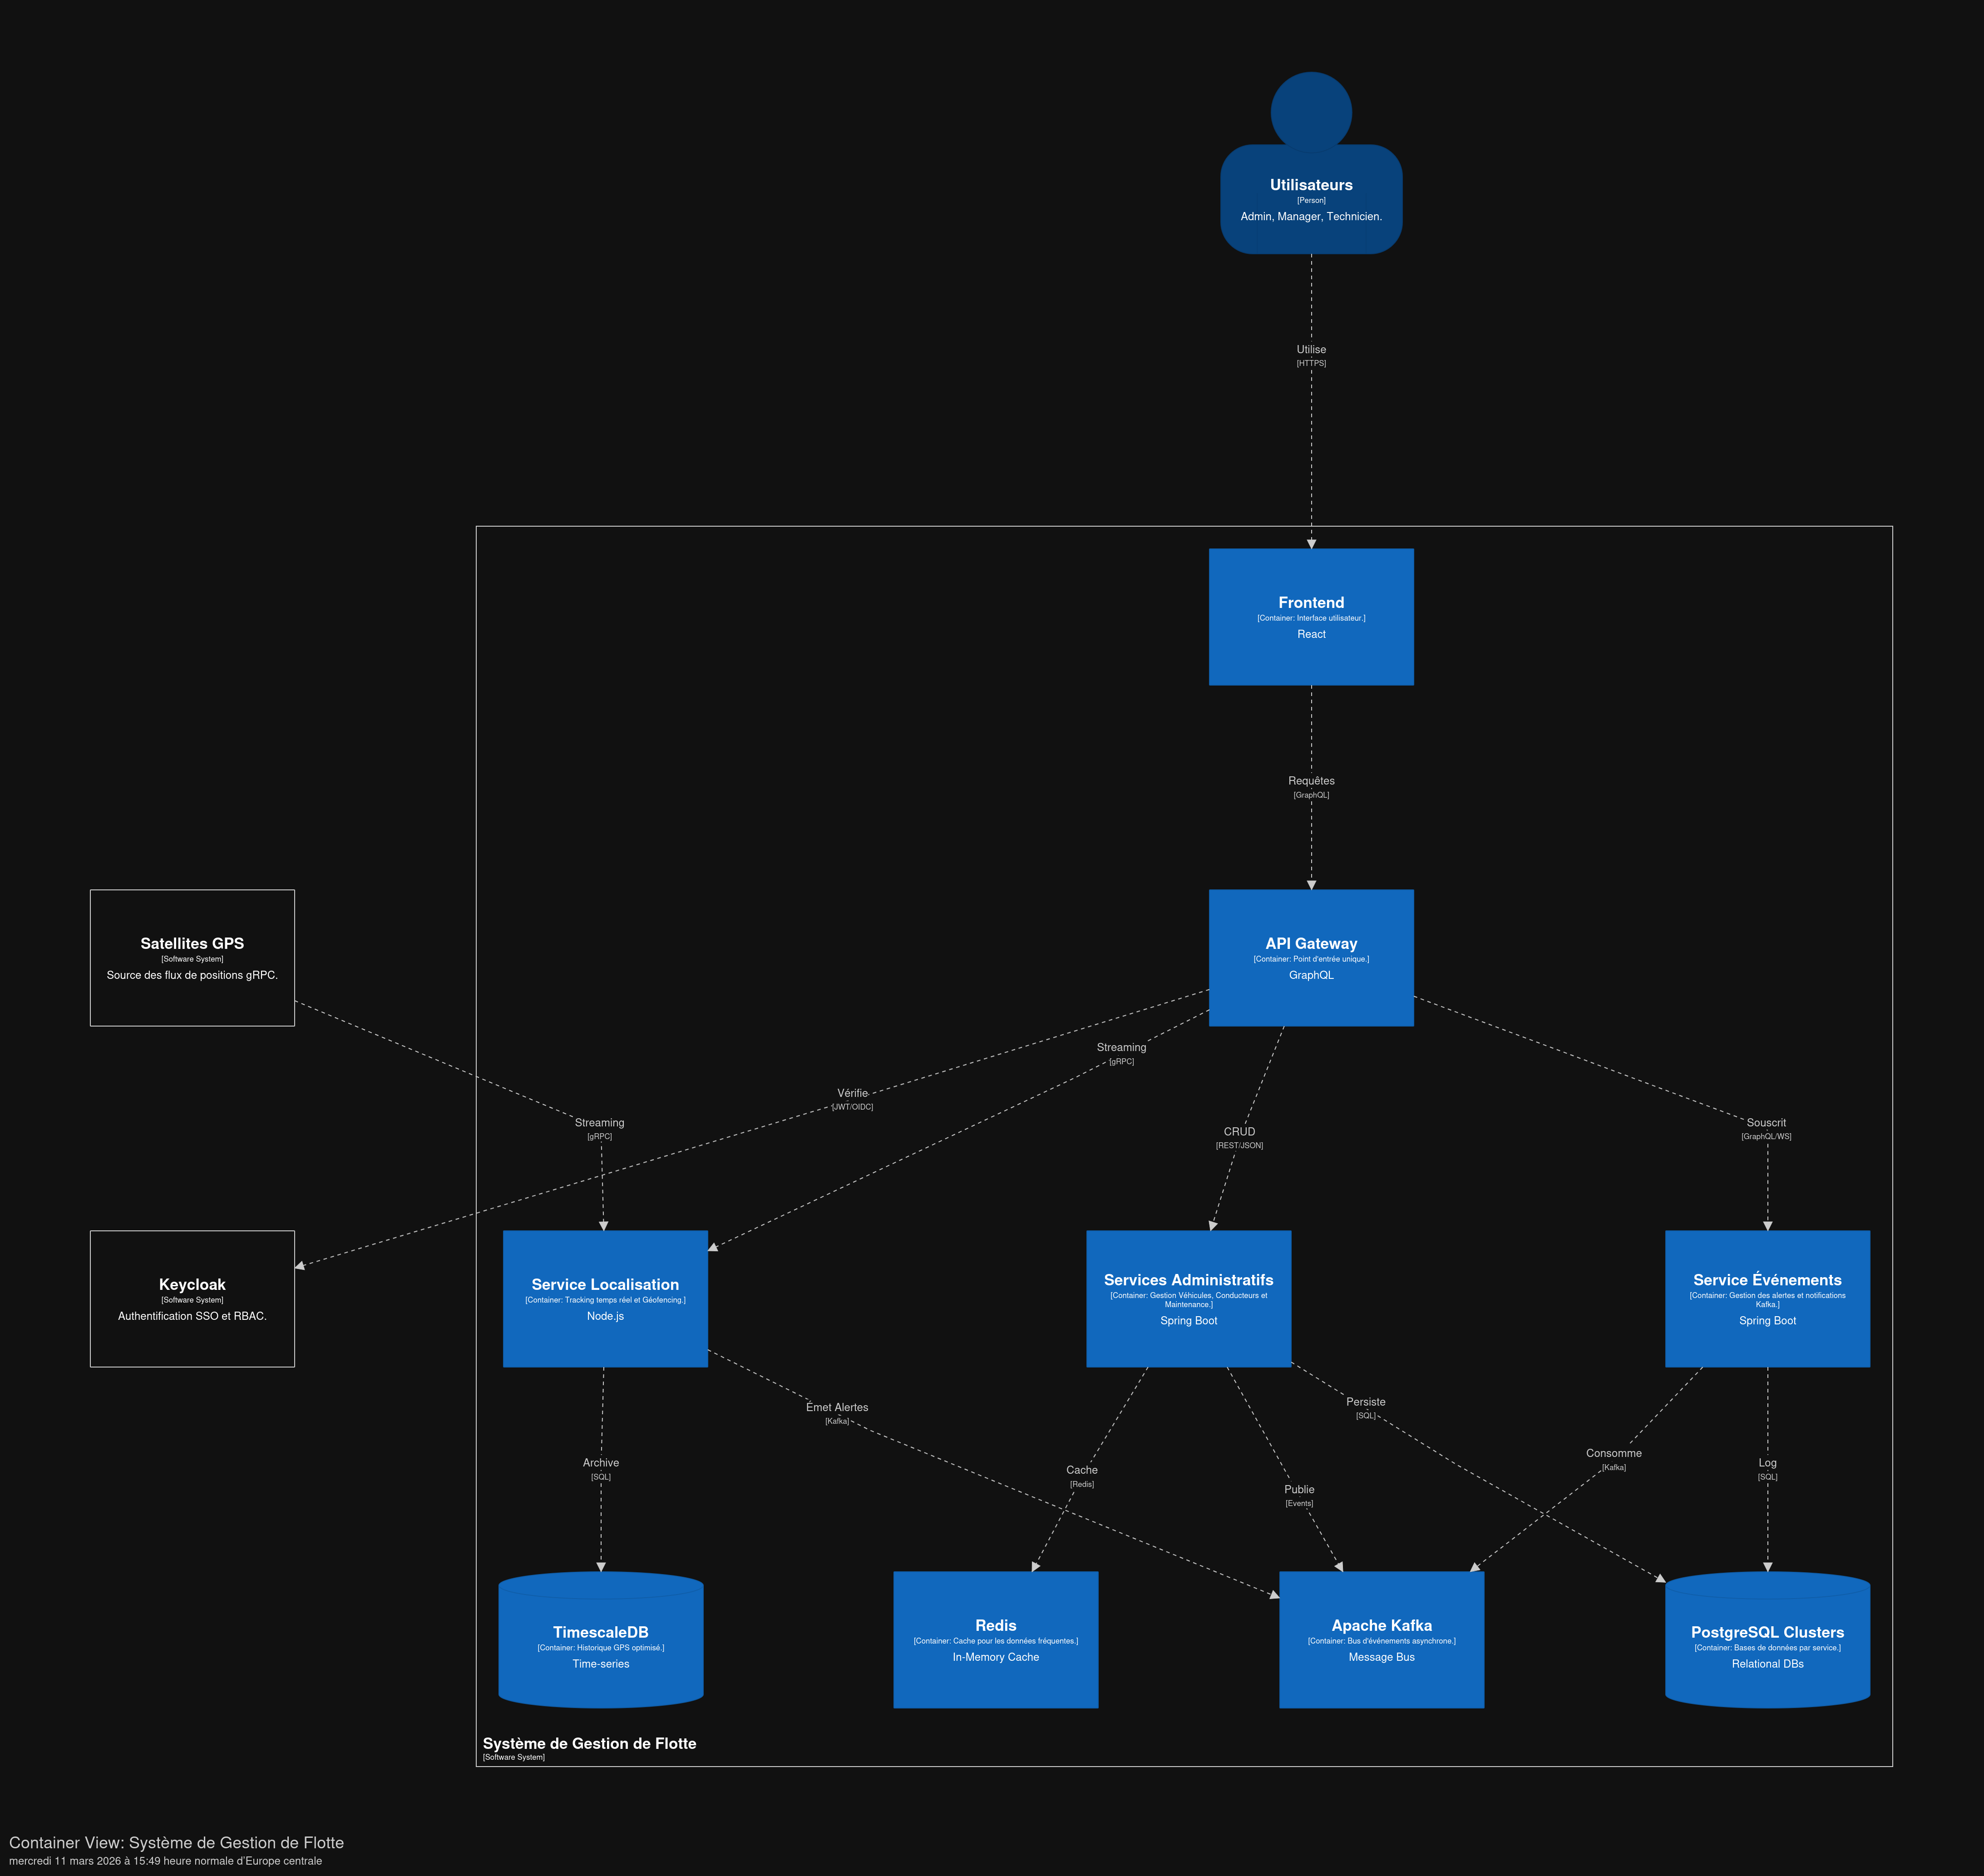
\includegraphics[width=0.95\linewidth]{C2.png}
  \centering{\tiny\color{muted} Architecture des conteneurs}
\end{minipage}

\vspace{4pt}
\ruledline

% ---- ADR ----

\section{ADR-001 — Services indépendants}

Le système doit faire trois choses à la fois : suivre les véhicules en direct, gérer les données administratives et envoyer des alertes. Ces trois besoins sont très différents et évolueront indépendamment.

\textbf{Décision :} séparer le système en trois parties indépendantes (Localisation, Administratif, Alertes), toutes accessibles depuis une seule adresse. \textbf{Avantage :} si une partie tombe en panne, les autres continuent de fonctionner. \textbf{Inconvénient :} un peu plus de choses à gérer au démarrage.



\section{ADR-002 — Protocole rapide pour le GPS}

Les boîtiers GPS envoient leur position plusieurs fois par seconde. Le protocole web classique n'est pas fait pour gérer autant de données en continu.

\textbf{Décision :} utiliser \textbf{gRPC}, un protocole conçu pour transmettre de grandes quantités de données rapidement. Les actions classiques (consulter, modifier) restent en HTTP normal. \textbf{Avantage :} les positions s'affichent sans délai perceptible. \textbf{Inconvénient :} une petite couche de traduction est nécessaire pour que le navigateur comprenne.



\section{ADR-003 — Alertes traitées sans bloquer le suivi}

Quand un véhicule dépasse une limite de vitesse ou entre dans une zone interdite, une alerte doit être envoyée. Cette étape ne doit pas ralentir le suivi GPS.

\textbf{Décision :} utiliser \textbf{Apache Kafka}, une file d'attente qui stocke les alertes à envoyer. Le suivi GPS dépose l'alerte, et le service d'envoi la traite quand il est prêt. \textbf{Avantage :} les deux parties travaillent sans se bloquer mutuellement, et aucune alerte n'est perdue. \textbf{Inconvénient :} un outil de plus à installer et surveiller.



\section{ADR-004 — Une base adaptée à chaque type de donnée}

Les positions GPS s'accumulent très rapidement, les données métier (véhicules, conducteurs) sont structurées et liées entre elles, et certaines informations sont consultées si souvent qu'elles doivent répondre en un instant.

\textbf{Décision :} utiliser trois bases de données, chacune adaptée à son rôle.

\begin{tabularx}{\linewidth}{lX}
  \toprule
  \small\textbf{Outil} & \small\textbf{Rôle} \\
  \midrule
  TimescaleDB  & Historique des positions GPS (conçu pour stocker efficacement des données qui arrivent en continu) \\
  PostgreSQL   & Véhicules, conducteurs, maintenances, alertes \\
  Redis        & Données consultées très souvent, stockées en mémoire pour répondre instantanément \\
  \bottomrule
\end{tabularx}



\section{ADR-005 — Connexion et droits centralisés}

Administrateurs, managers et techniciens n'ont pas accès aux mêmes fonctionnalités. Il faut un moyen simple de gérer qui peut faire quoi, sans le répéter dans chaque partie du système.

\textbf{Décision :} utiliser \textbf{Keycloak}, un outil gratuit qui centralise la gestion des comptes et des droits. L'utilisateur se connecte une seule fois et peut accéder à toutes les parties du système selon son rôle. \textbf{Avantage :} les droits sont gérés en un seul endroit. \textbf{Inconvénient :} si cet outil est en panne, plus personne ne peut se connecter — il doit donc toujours être disponible.

\vspace{3pt}
\ruledline


% ---- SCHEMAS BDD ----
{\small\color{muted} Schémas de base de données (PostgreSQL)}\\[4pt]
\begin{minipage}[t]{0.48\linewidth}
  \centering
  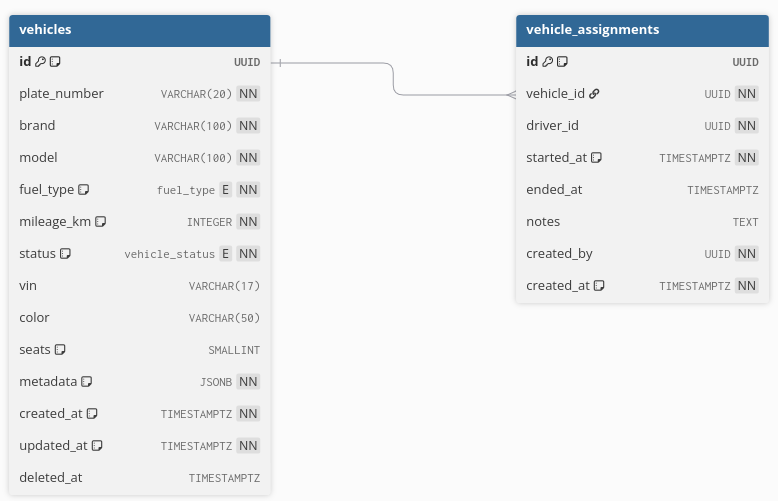
\includegraphics[width=0.75\linewidth]{b1.png}\\[4pt]
  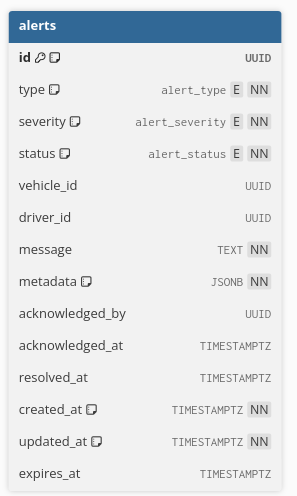
\includegraphics[width=0.75\linewidth]{b3.png}
\end{minipage}
\hfill
\begin{minipage}[t]{0.48\linewidth}
  \centering
  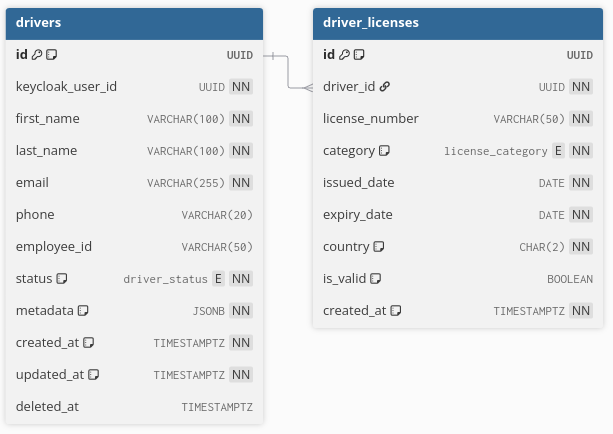
\includegraphics[width=0.75\linewidth]{b2.png}\\[4pt]
  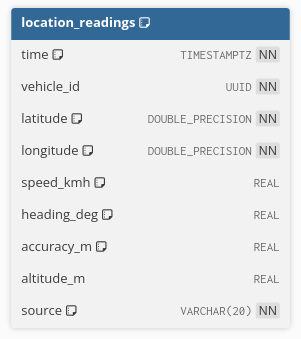
\includegraphics[width=0.75\linewidth]{b4.png}
\end{minipage}

\end{document}